\chapter{ผลการทดสอบแบตเตอรี่ตามมาตรฐานและผลการทดสอบอื่นๆ}
ในบทนี้จะแสดงถึงผลการทดสอบแบตเตอรี่ตามมาตรฐาน UN ECE R136 ในหัวข้อการทดสอบการป้องกันการดิสชาร์จเกินและในหัวข้อการทดสอบการป้องกันการชาร์จเกิน สำหรับการทดสอบอื่นๆคือ
การทดสอบอัตรากระแสที่มีผลต่อความจุของแบตเตอรี่ การทดสอบการวัดความต้านทานภายใน และสุดท้ายการทดสอบระยะเวลาการพักของแบตเตอรี่ซึ่งการทดสอบทั้งหมดนี้จะถูกทดสอบด้วยเครื่องทดสอบแบตเตอรี่
Chroma model 17020 ดังรูปที่\ref{fig:Chroma model 17020}
%==========================================================================================
\section{การทดสอบตามมาตรฐาน UN ECE R136}
ในหัวข้อการทดสอบนี้จะทดสอบแบตเตอรี่ด้วยกันทั้งสิ้น 3 โมดูลคือ
\begin{itemize}
 {\item แบตเตอรี่สำหรับจักรยานยนต์ไฟฟ้า 72V 30Ah ดังรูปที่\ref{fig:Battery_72V30Ah}}
 {\item แบตเตอรี่สำหรับรถสามล้อไฟฟ้า 72V 60Ah ดังรูปที่\ref{fig:Battery_72V60Ah}}
 {\item แบตเตอรี่ 72V 72Ah ดังรูปที่\ref{fig:Battery_72V72Ah} ซึ่งมีคุณสมบัติดังตารางที่\ref{table:spec_72V72Ah}}
\end{itemize}
และทดสอบด้วยกันทั้ง 2 หัวข้อจาก 10 หัวข้อจากมาตรฐาน UN ECE R136 คือ
\begin{itemize}
 {\item การทดสอบการป้องกันการชาร์จเกิน โดยการทดสอบนี้จะดำเนินขั้นตอนการทดสอบตาม\\บทที่3 หัวข้อที่3.3.1}
 {\item การทดสอบการป้องกันการดิสชาร์จเกิน โดยการทดสอบนี้จะดำเนินขั้นตอนการทดสอบตามบทที่3 หัวข้อที่3.3.2}
\end{itemize}
สำหรับวงจรการทดสอบการป้องกันการชาร์จเกินจะเป็นดังรูปที่\ref{fig:Test_Setup} และวงจรการทดสอบการป้องกันการดิสชาร์จเกินจะเป็นดังรูปที่\ref{fig:Test_Setup2}
ซึ่งจากขั้นตอนการทดสอบจะต้องชาร์จหรือดิสชาร์จด้วยอัตรากระแสที่คงที่และวัดค่ากระแสและแรงดันตลอดการทดสอบซึ่งการชาร์จหรือดิสชาร์จ การวัดค่ากระแสและแรงดัน และการบันทึกค่านั้นทั้งหมด
จะทำได้ด้วยเครื่องทดสอบแบตเตอรี่ \\Chroma model 17020 
\begin{center}
\begin{figure}[H]
	\makebox[\textwidth]{
	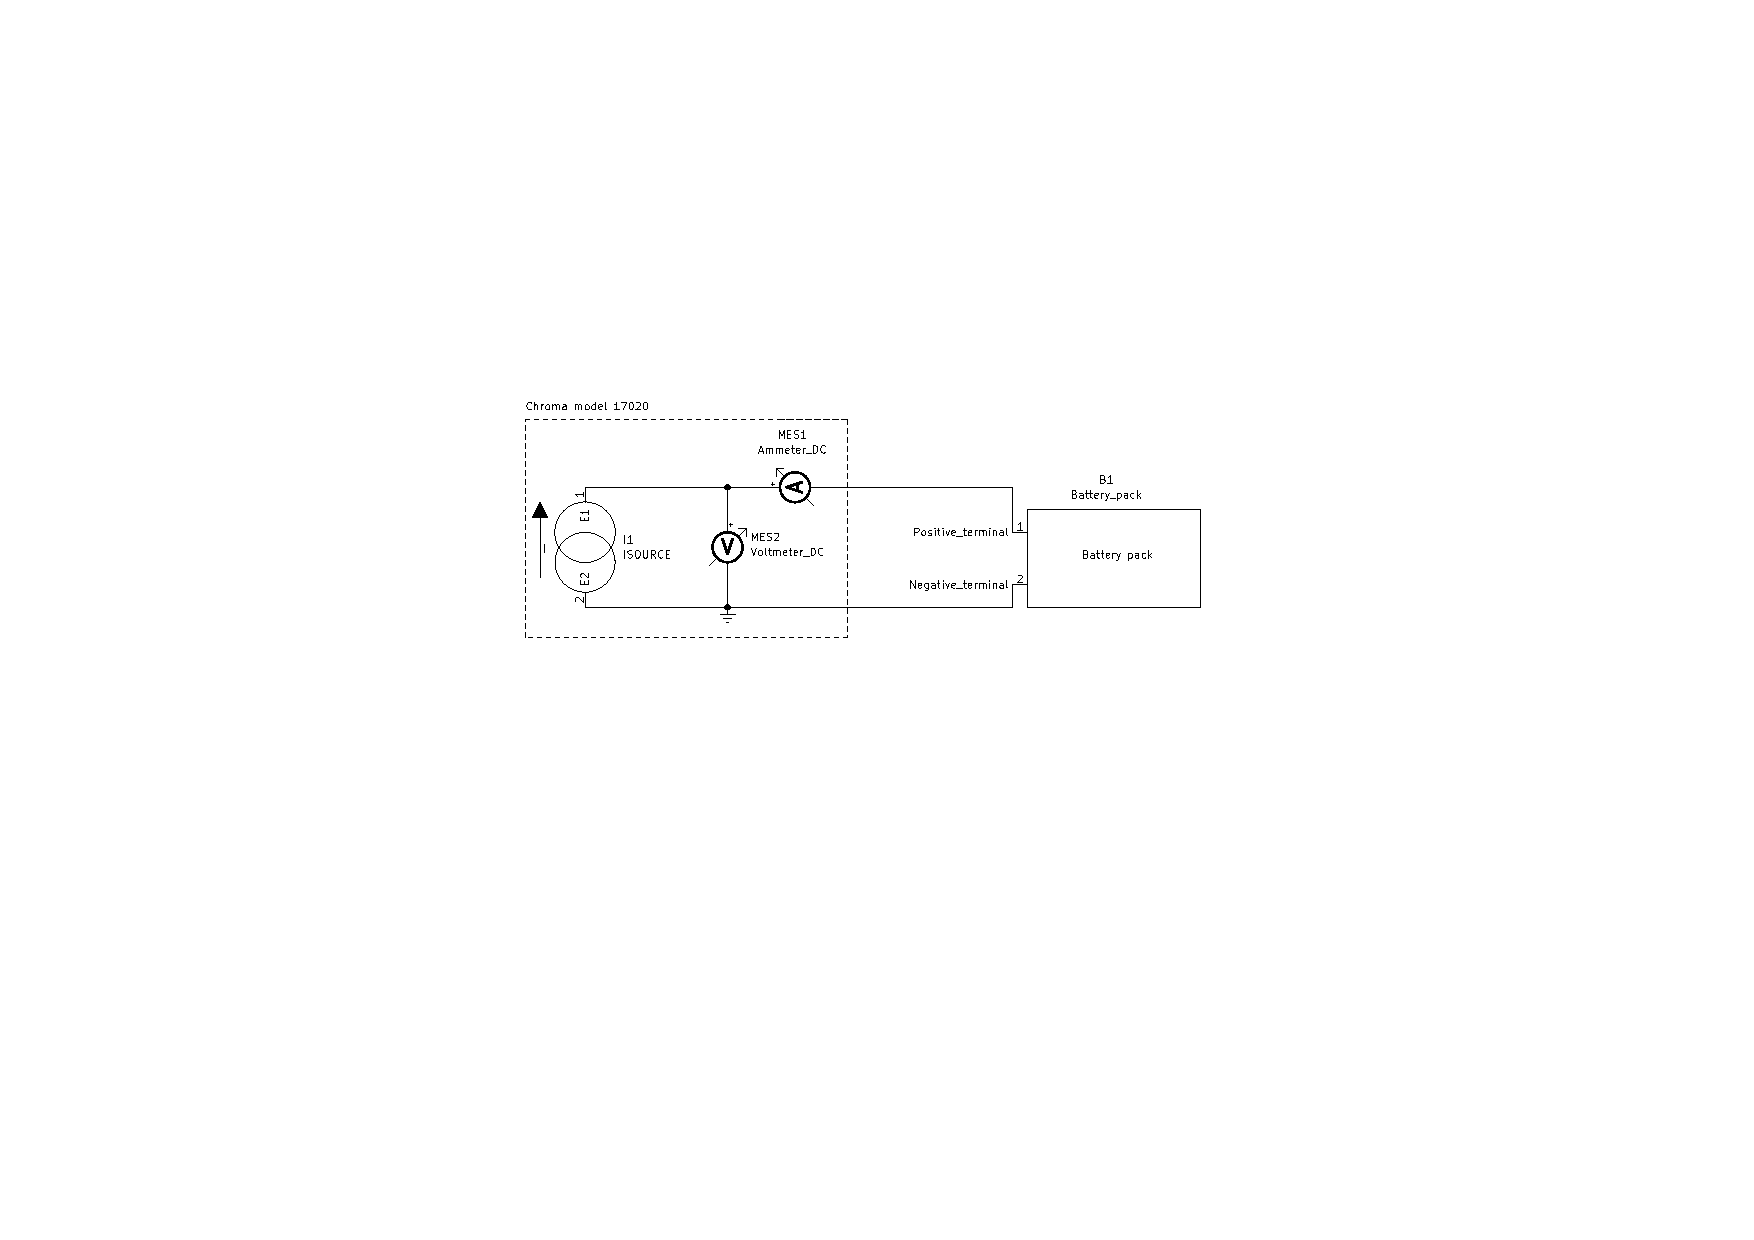
\includegraphics[width=0.8\paperwidth]{Chapters/img/Test_Setup.pdf}}
		\centering
		\captionsetup{justification=centering,margin=2cm}
		\caption{รูปวงจรการทดสอบการป้องกันการชาร์จเกิน}
		\label{fig:Test_Setup}
	\end{figure}
	\begin{figure}[H]
	\makebox[\textwidth]{
	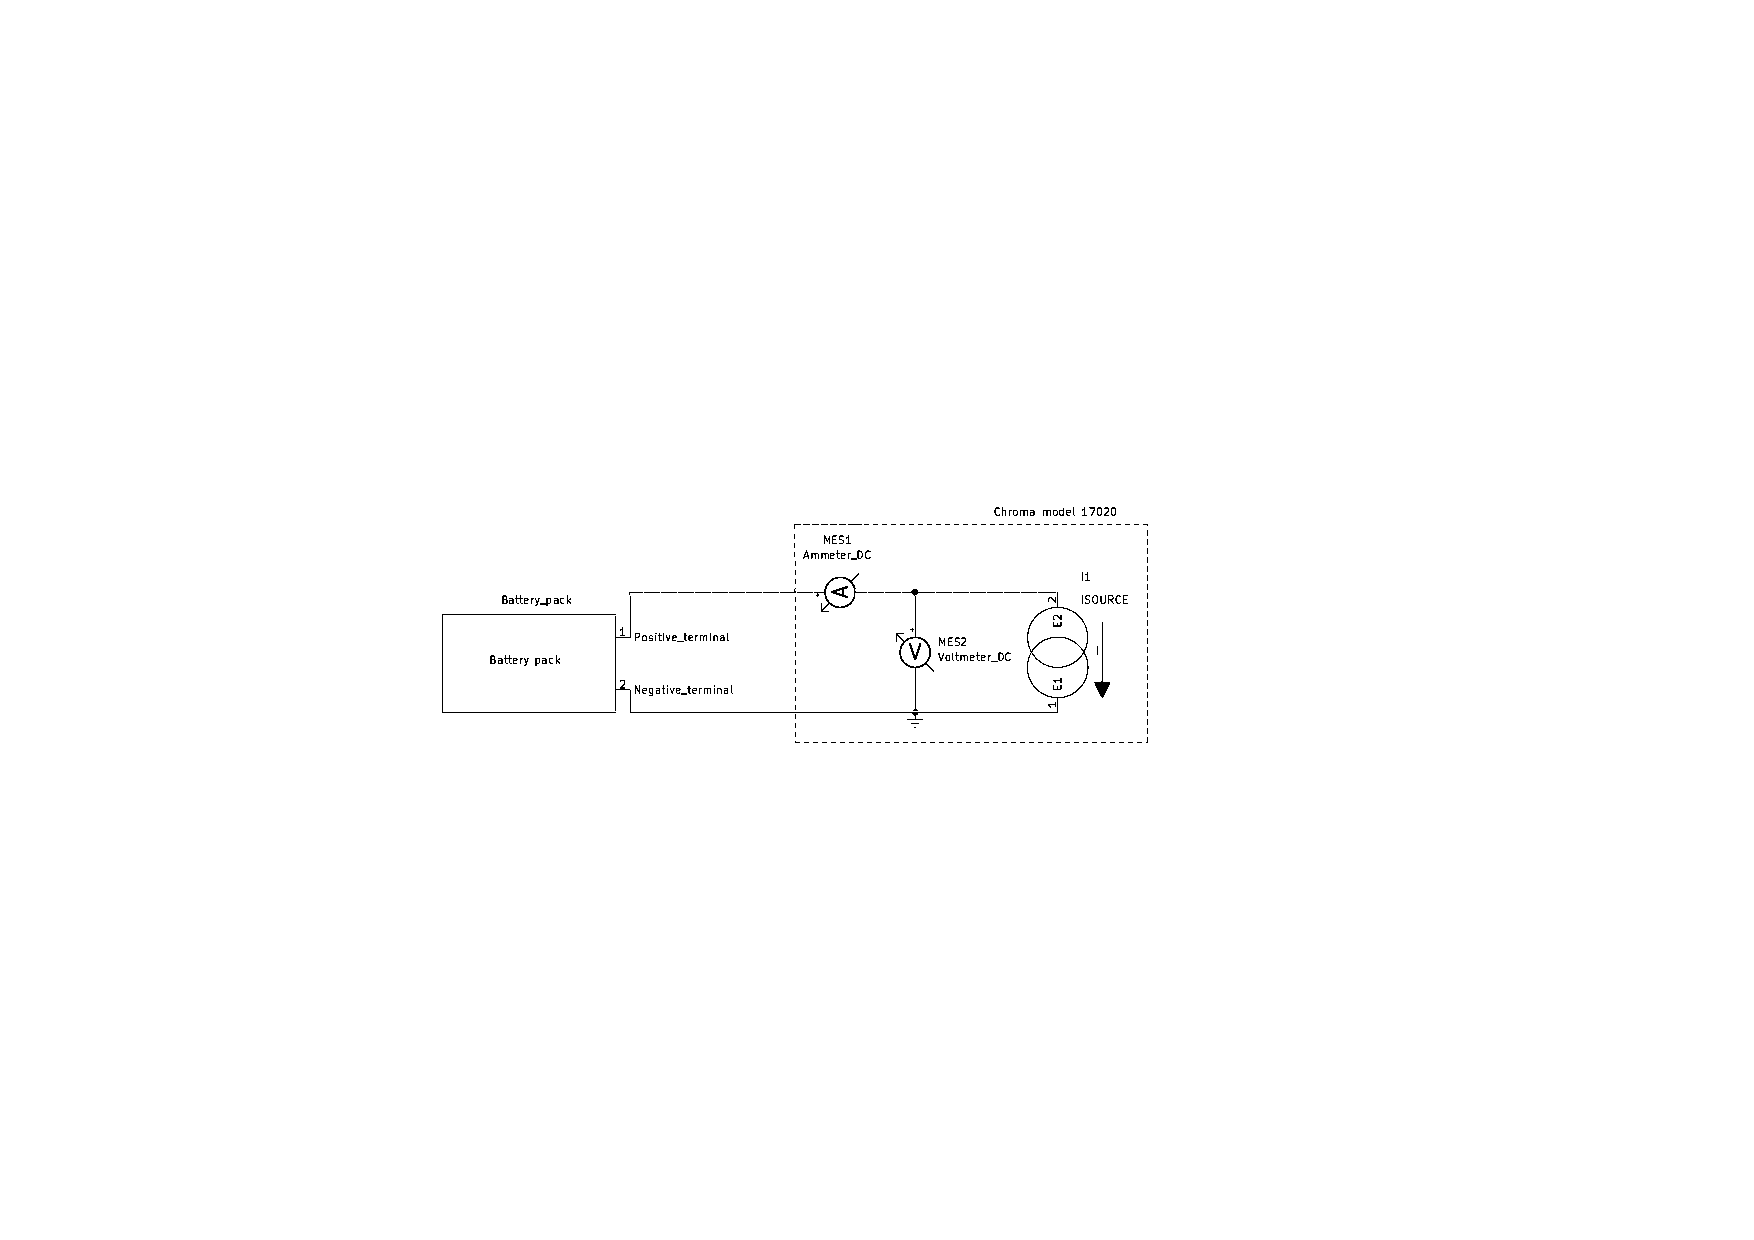
\includegraphics[width=0.8\paperwidth]{Chapters/img/Test_Setup2.pdf}}
		\centering
		\captionsetup{justification=centering,margin=2cm}
		\caption{รูปวงจรการทดสอบการป้องกันการดิสชาร์จเกิน}
		\label{fig:Test_Setup2}
	\end{figure}
\end{center}
%==========================================================================================
\section{การทดสอบอื่นๆ}
ในหัวข้อการทดสอบนี้จะทดสอบแบตเตอรี่ด้วยกันทั้งสิ้น 3 โมดูลคือ
\begin{itemize}
 {\item แบตเตอรี่สำหรับจักรยานยนต์ไฟฟ้า 72V 30Ah ดังรูปที่\ref{fig:Battery_72V30Ah}}
 {\item แบตเตอรี่สำหรับรถสามล้อไฟฟ้า 72V 60Ah ดังรูปที่\ref{fig:Battery_72V60Ah}}
 {\item แบตเตอรี่ 72V 72Ah ดังรูปที่\ref{fig:Battery_72V72Ah} ซึ่งมีคุณสมบัติดังตารางที่\ref{table:spec_72V72Ah}}
\end{itemize}
และทดสอบด้วยกันทั้งหมด 3 หัวซึ่งโดยการทดสอบนี้จะดำเนินตามขั้นตอนการทดสอบในบทที่ 3 หัวข้อที่ 3.3.3 คือ
\begin{itemize}
 {\item การทดสอบอัตรากระแสที่มีผลต่อความจุของแบตเตอรี่}
 {\item การทดสอบระยะเวลาการพักของแบตเตอรี่}
 {\item การทดสอบการวัดความต้านทานภายในของแบตเตอรี่}
\end{itemize}
สำหรับวงจรการทดสอบอัตรากระแสที่มีผลต่อความจุของแบตเตอรี่และวัดความต้านทานภายในจะใช้วงจรดังรูปที่\ref{fig:Test_Setup2}และสำหรับวงจรการทดสอบการวัดความต้านทานภายในจะใช้วงจรดังรูปที่
\ref{fig:Test_Setup3}
\begin{center}
	\begin{figure}[H]
	\makebox[\textwidth]{
	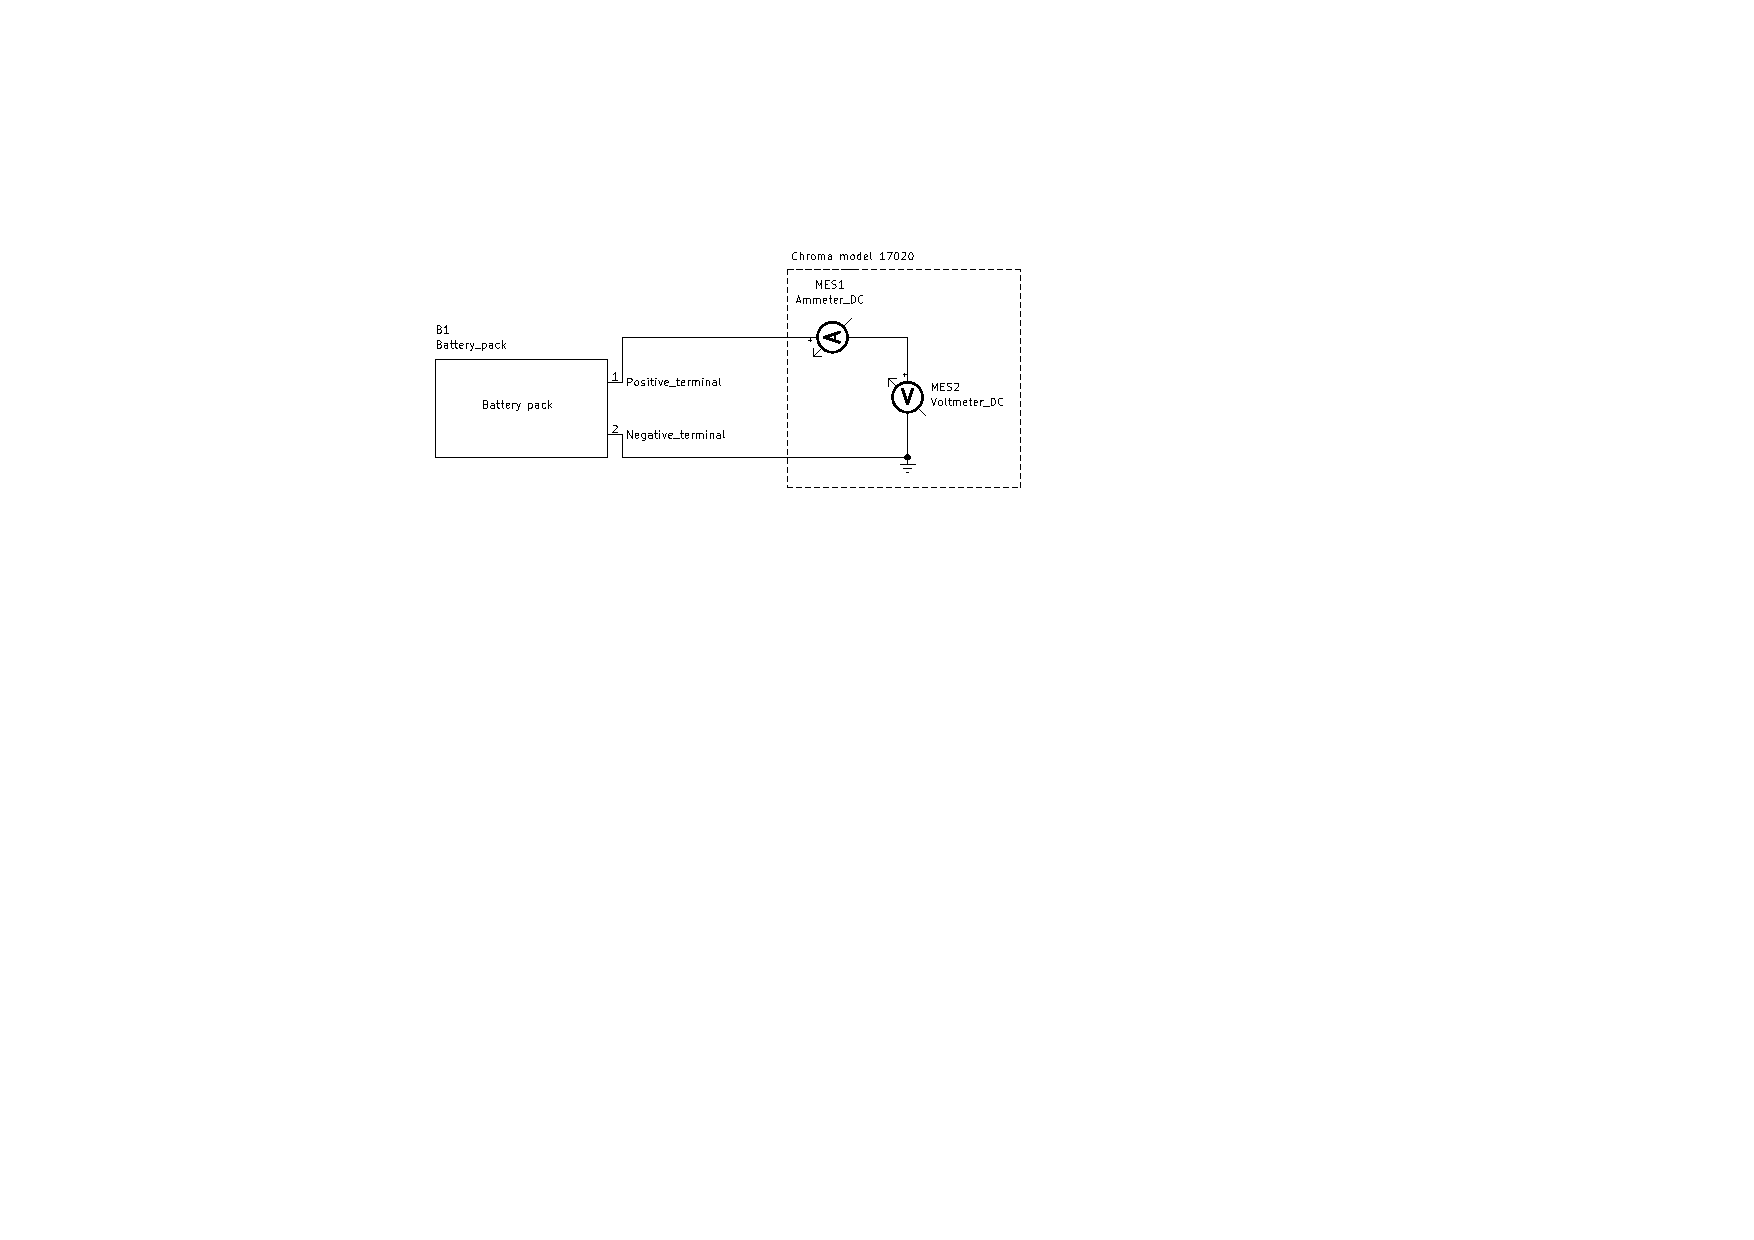
\includegraphics[width=0.8\paperwidth]{Chapters/img/Test_Setup3.pdf}}
		\centering
		\captionsetup{justification=centering,margin=2cm}
		\caption{รูปวงจรการทดสอบระยะเวลาพักของแบตเตอรี่}
		\label{fig:Test_Setup3}
	\end{figure}
\end{center}
ซึ่งผลการทดสอบทั้งหมดจะมีดังนี้ 
%-------------------------------------------
\pagebreak
\subsection{ผลการทดสอบการป้องกันการชาร์จเกิน}
สำหรับการทดสอบการป้องกันการชาร์จเกินของแบตเตอรี่สำหรับจักรยานยนต์ไฟฟ้า 72V 30Ah มีดังนี้
\begin{center}
	\begin{figure}[H]
	\makebox[\textwidth]{
	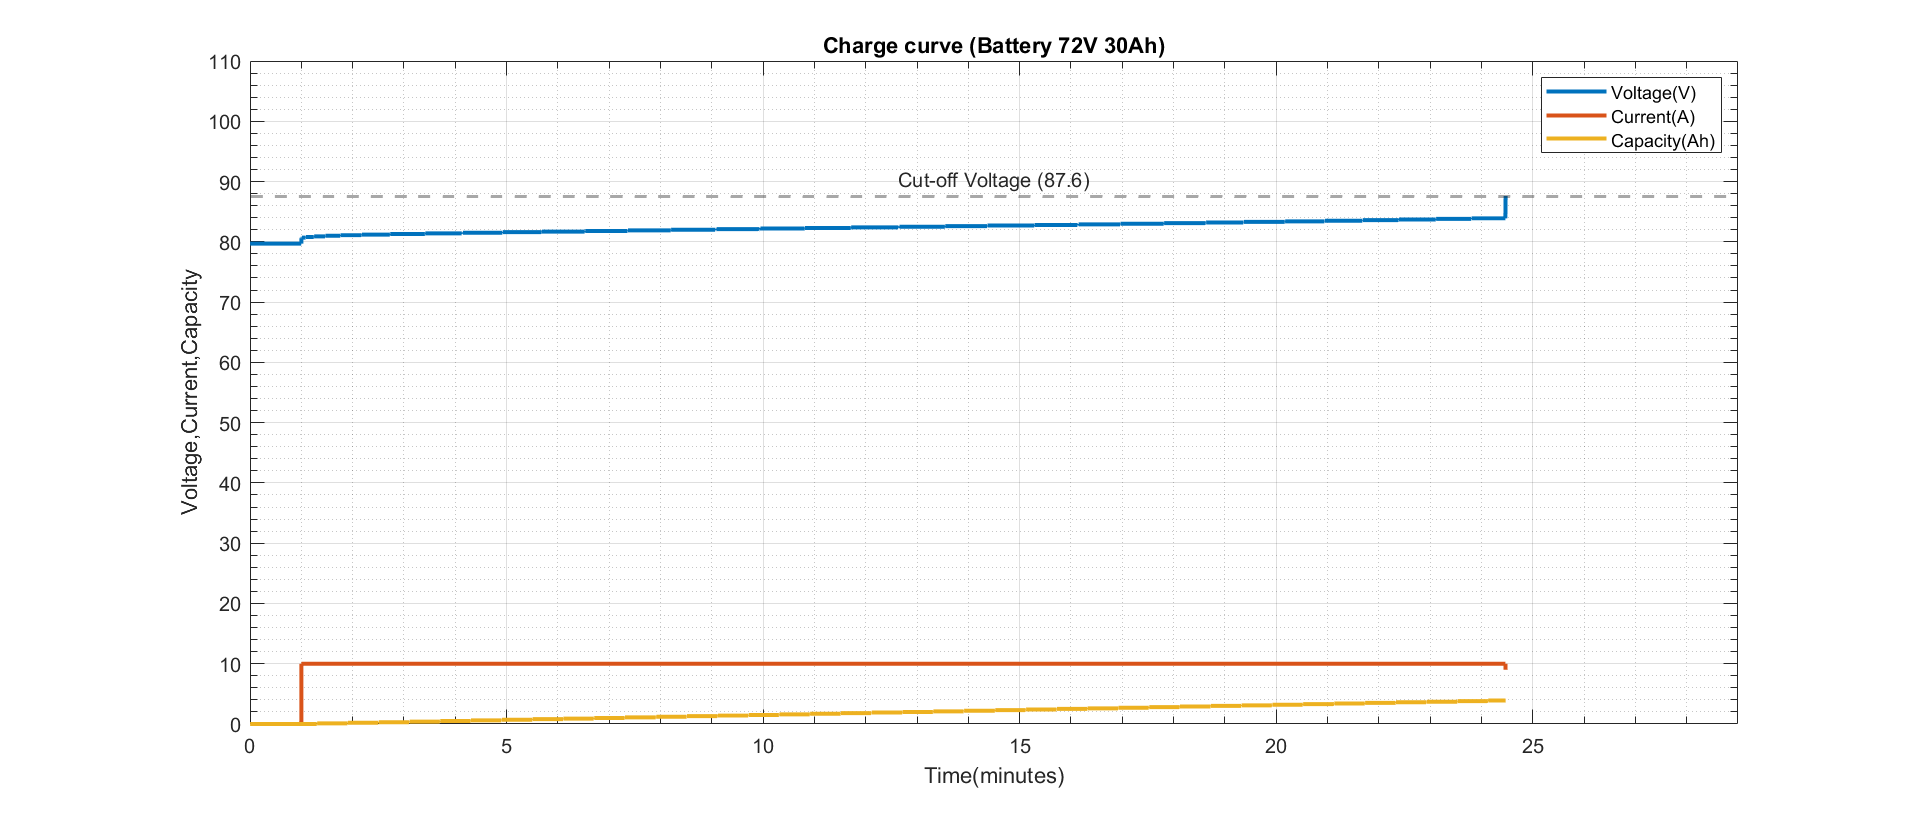
\includegraphics[width=\paperwidth]{Chapters/img/Result/Charge curve 72V30Ah_OV.png}}
		\centering
		\captionsetup{justification=centering,margin=2cm}
		\caption{กราฟการทดสอบการป้องกันการชาร์จเกินของแบตเตอรี่ 72V30Ah}
	\end{figure}
\end{center}
จากการทดสอบพบว่าแบตเตอรี่สำหรับจักรยานยนต์ไฟฟ้าในระหว่างการทดสอบไม่มีการรั่วไหลของ\\อิเล็กโทรไลต์ ไม่มีการแตกหักหรือฉีกขาด ไม่เกิดเพลิงไหม้ และไม่เกิดการระเบิด
โดยการทดสอบการชาร์จนี้ถูกขัดจังหวะโดยระบบการจัดการแบตเตอรี่(BMS)ของโมดูลแบตเตอรี่นี้เองโดยขัดจังหวะเมื่อแรงดันของโมดูลแบตเตอรี่อยู่ที่ 83.9V
ซึ่งจากการตั้งค่าการป้องกันการชาร์จเกินของระบบการจัดการแบตเตอรี่ของโมดูลแบตเตอรี่ 72V30Ah ซึ่งเป็นไปดังรูปที่\ref{fig:BMS_Setting}
ซึ่งจะเห็นได้ว่าแรงดันที่ระบบการจัดการแบตเตอรี่นั้นได้ขัดจังหวะการชาร์จมีความใกล้เคียงกับที่ได้ตั้งค่าไว้มากที่ 4.2V ต่อเซลล์(โดยแบตเตอรี่โมดูลนี้มี 20 เซลล์)หรือก็คือ 84V สำหรับแบตเตอรี่โมดูลนี้
โดยมีความคลาดเคลื่อนอยู่ที่ 0.1V หรือคิดเป็น 0.119\% ของแรงดันที่ได้ตั้งค่าไว้หลังจากที่หยุดการชาร์จจากนั้นผู้ทดสอบได้ทำการสังเกตแบตเตอรี่เป็นระยะเวลา 1 
ชั่วโมงพบว่าแบตเตอรี่ยังคงสภาพปกติและยังคงสามารถใช้งานได้
ซึ่งจะสังเกตได้ว่าโมดูลแบตเตอรี่นี้หลังจากการทดสอบการป้องกันการชาร์จเกินตามมาตรฐาน UN ECE R136 พบว่าผ่านการทดสอบโดยที่แบตเตอรี่นี้ยังสามารถใช้งานได้อย่างปกติ
\newpage
ผลจากการทดสอบแบตเตอรี่สำหรับรถสามล้อไฟฟ้า 72V 60Ah มีดังนี้
\begin{center}
	\begin{figure}[H]
	\makebox[\textwidth]{
	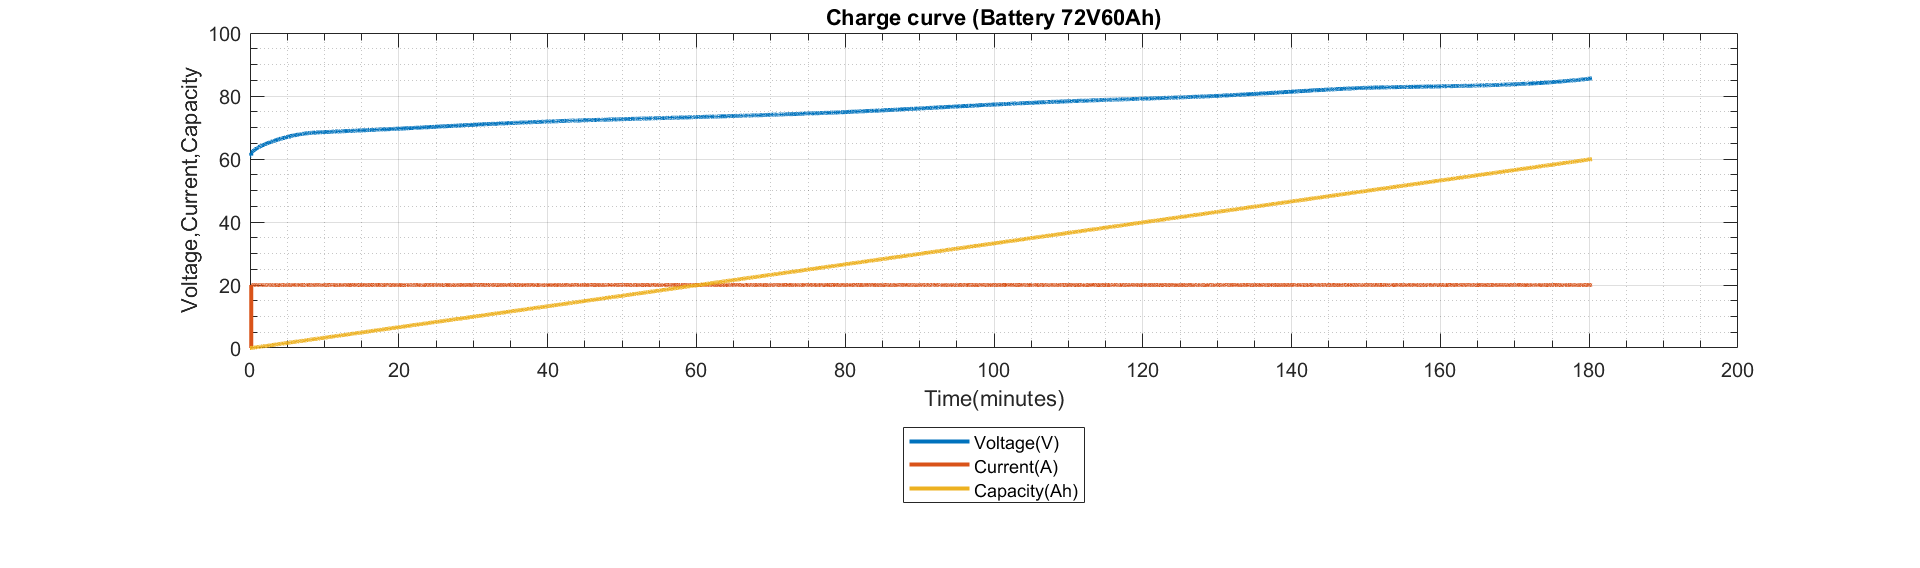
\includegraphics[width=\paperwidth]{Chapters/img/Result/Charge curve 72V60Ah.png}}
		\centering
		\captionsetup{justification=centering,margin=2cm}
		\caption{กราฟการทดสอบการป้องกันการชาร์จเกินของแบตเตอรี่ 72V60Ah}
	\end{figure}
\end{center}
จากการทดสอบพบว่าแบตเตอรี่สำหรับรถสามล้อไฟฟ้าระหว่างการทดสอบไม่มีการรั่วไหลของอิเล็ก-โทรไลต์ ไม่มีการแตกหักหรือฉีกขาด ไม่เกิดเพลิงไหม้ และไม่เกิดการระเบิด
แต่การทดสอบนั้นถูกขัดจังหวะโดยผู้ทดสอบเองโดยขัดจังหวะที่แรงดันของโมดูลแบตเตอรี่อยู่ที่ 85.6V เนื่องจากหากดำเนินการทดสอบต่อไปอาจจะทำให้เกิดความเสียหายกับแบตเตอรี่และอุปกรณ์การทดสอบได้ซึ่ง
หลังจากที่หยุดการชาร์จผู้ทดสอบได้ทำการสังเกตแบตเตอรี่เป็นระยะเวลา 1 ชั่วโมงพบว่าแบตเตอรี่ยังคงสภาพปกติและยังคงสามารถใช้งานได้ซึ่งหลังจากที่ได้ทดสอบการป้องกันการชาร์จเกินโมดูลแบตเตอรี่นี้ตามมาตรฐาน
UN ECE R136 จากการที่การทดสอบนี้มีปัญหาเนื่องจากไม่ทราบข้อมูลคุณสมบัติของแบตเตอรี่อย่างครบถ้วนจึงทำให้ไม่สามารถทราบถึงขีดจำกัดของโมดูลแบตเตอรี่นี้ทำให้ไม่สามารถสรุปได้ว่าโมดูลแบตเตอรี่นี้
ผ่านการทดสอบหรือไม่
\newpage
ผลจากการทดสอบแบตเตอรี่ 72V 72Ah มีดังนี้
\begin{center}
	\begin{figure}[H]
	\makebox[\textwidth]{
	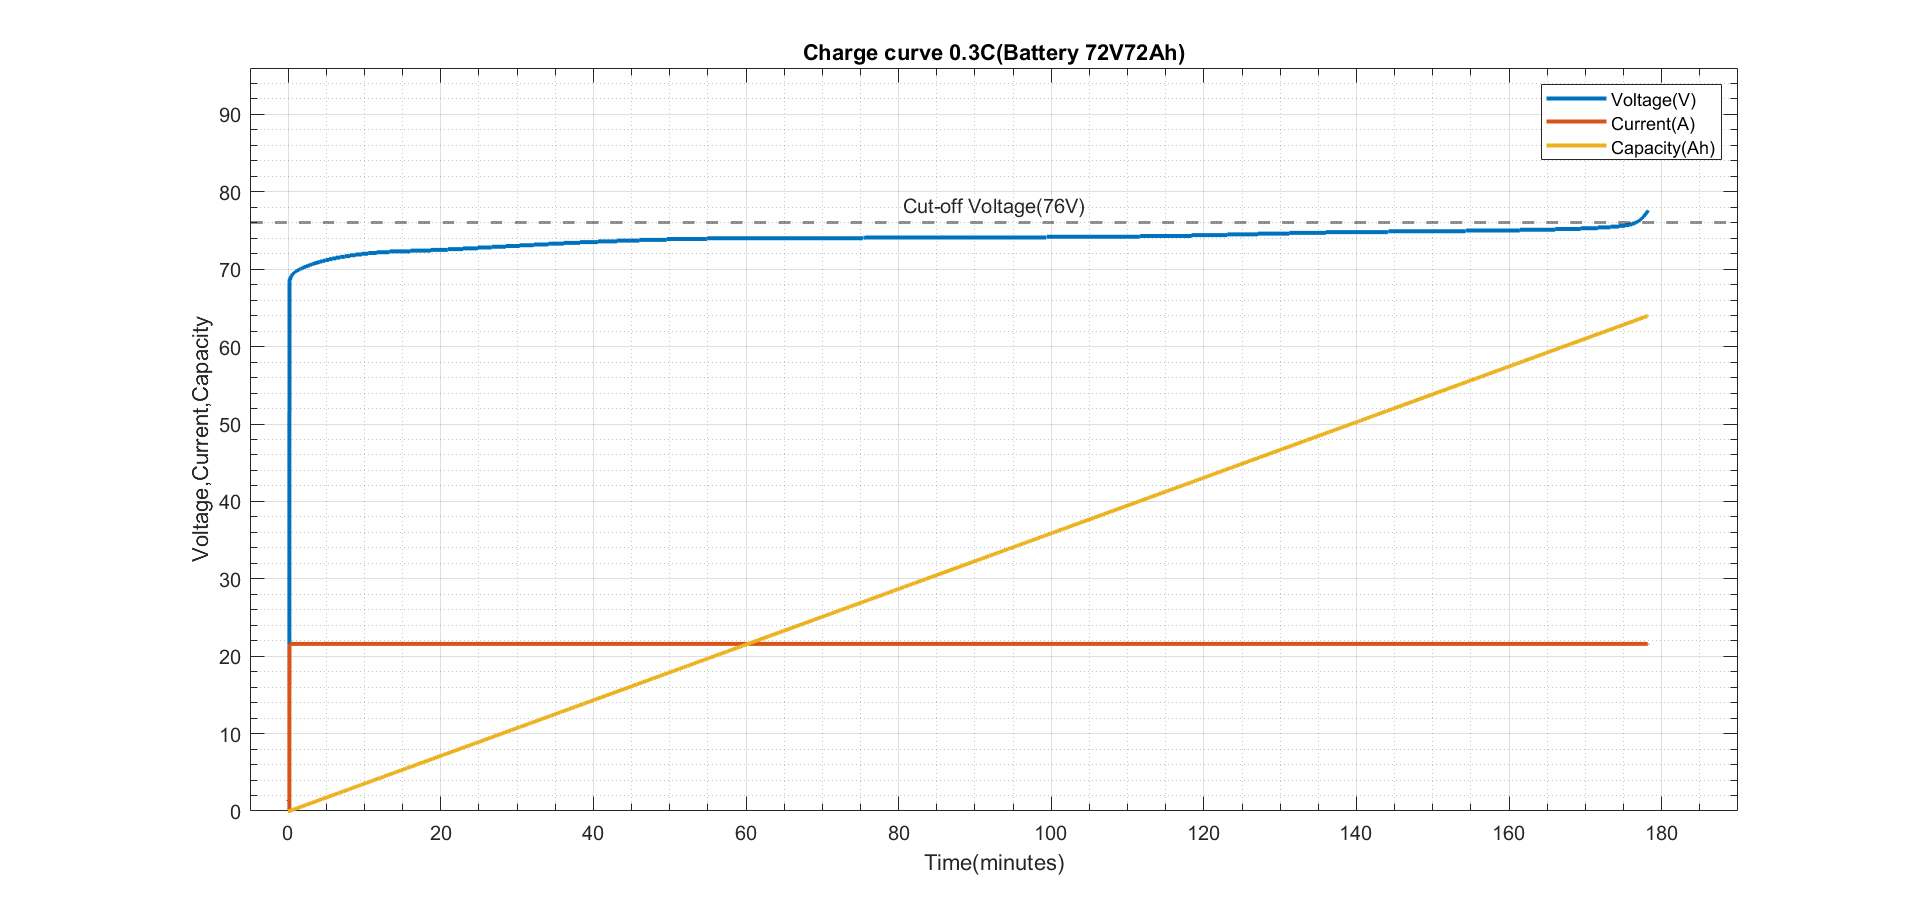
\includegraphics[width=\paperwidth]{Chapters/img/Result/Charge curve 0.3C 72V72Ah.png}}
		\centering
		\captionsetup{justification=centering,margin=2cm}
		\caption{กราฟการทดสอบการป้องกันการชาร์จเกินของแบตเตอรี่ 72V72Ah}
	\end{figure}
\end{center}
จากการทดสอบพบว่าแบตเตอรี่สำหรับรถสามล้อไฟฟ้าระหว่างการทดสอบไม่มีการรั่วไหลของอิเล็กโทรไลต์ ไม่มีการแตกหักหรือฉีกขาด ไม่เกิดเพลิงไหม้ และไม่เกิดการระเบิด
โดยการทดสอบการชาร์จนี้ถูกขัดจังหวะโดยระบบการจัดการแบตเตอรี่(BMS)ของโมดูลแบตเตอรี่นี้เองโดยขัดจังหวะเมื่อแรงดันของโมดูลแบตเตอรี่อยู่ที่ 77.6V
หลังจากที่หยุดการชาร์จจากนั้นผู้ทดสอบได้ทำการสังเกตแบตเตอรี่เป็นระยะเวลา 1 ชั่วโมงพบว่าแบตเตอรี่ยังคงสภาพปกติและยังคงสามารถใช้งานได้
หลังจากที่ได้ทดสอบแบตเตอรี่โมดูลนี้ตามมาตรฐาน UN ECE R136 ในหัวข้อการทดสอบการป้องกันการชาร์จเกินพบว่าโมดูลแบตเตอรี่นี้ผ่านการทดสอบโดยการที่ระบบการจัดการแบตเตอรี่
ของแบตเตอรี่โมดูลนี้ทำการขัดจังหวะการชาร์จโดยจากตารางคุณสมบัติของระบบการจัดการแบตเตอรี่นี้ดังรูปที่\ref{fig:BMS_Setting2}จะเห็นได้ว่าแรงดันที่ระบบการจัดการแบตเตอรี่นี้
จะทำการขัดจังหวะการชาร์จจะอยู่ที่ $3.55\pm 0.05V$ ต่อเซลล์(โดยแบตเตอรี่โมดูลนี้มี 22 เซลล์)หรือก็คือ $78.1\pm 1.1V$ สำหรับโมดูลแบตเตอรี่นี้
ซึ่งจากการทดสอบแล้วจะเห็นได้ว่าแบตเตอรี่โมดูลนี้ถูกขัดจังหวะการชาร์จที่ 77.6V ซึ่งจะสังเกตได้ว่าระบบการจัดการแบตเตอรี่นี้ทำงานได้อย่างปกติโดยหลังจากการทดสอบนี้พบว่าแบตเตอรี่โมดูลนี้ผ่านการทดสอบตามาตรฐาน
UN ECE R136 ในหัวข้อการทดสอบการป้องกันการชาร์จเกินซึ่งโมดูลแบตเตอรี่นี้ยังสามารถใช้งงานได้อย่างปกติ
%----------------------------------------------------------------------------------
\subsection{ผลการทดสอบการป้องกันการดิสชาร์จเกิน}
สำหรับการทดสอบการป้องกันการดิสชาร์จเกินของแบตเตอรี่สำหรับจักรยานยนต์ไฟฟ้า 72V 30Ah มีดังนี้
\begin{center}
	\begin{figure}[H]
	\makebox[\textwidth]{
	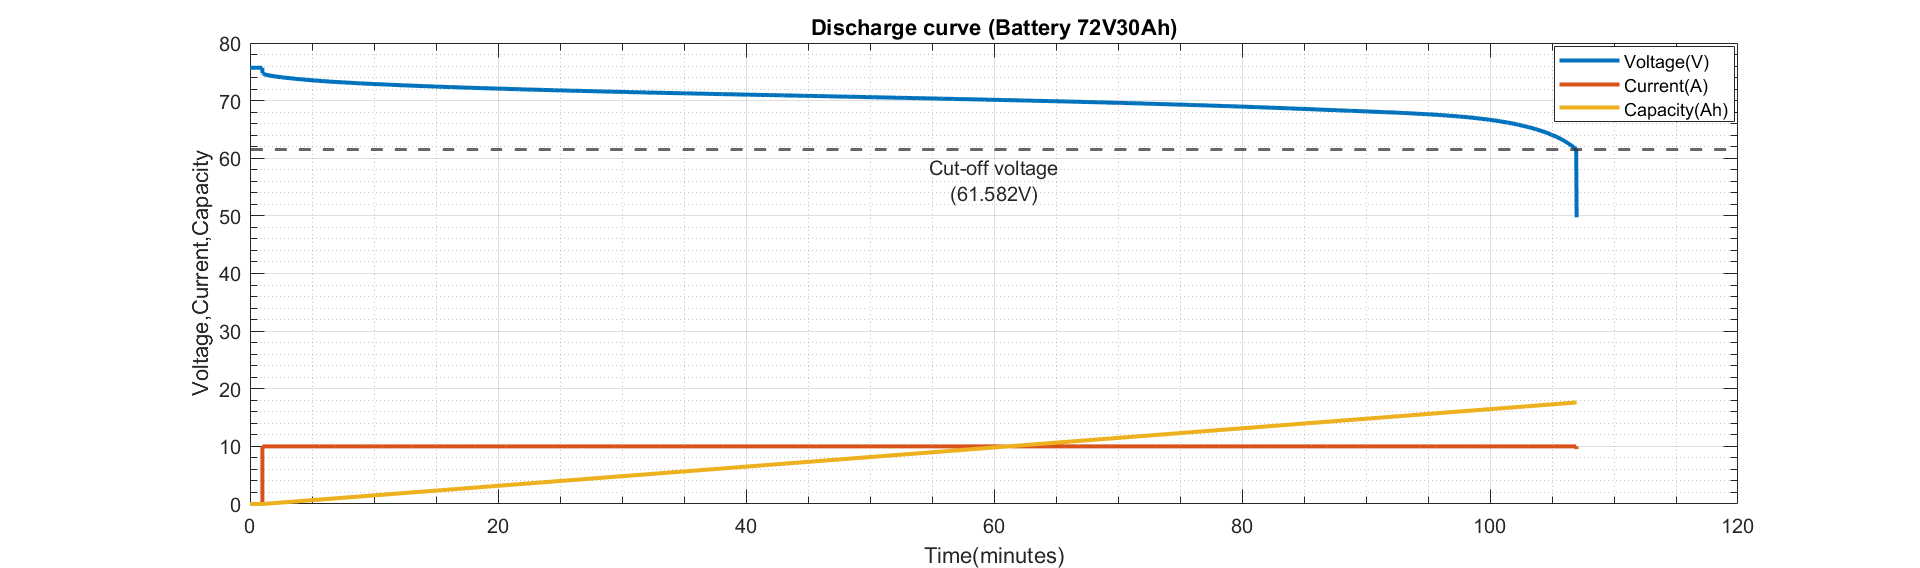
\includegraphics[width=\paperwidth]{Chapters/img/Result/Discharge curve 72V30Ah.png}}
		\centering
		\captionsetup{justification=centering,margin=2cm}
		\caption{กราฟการทดสอบการป้องกันการดิสชาร์จเกินของแบตเตอรี่ 72V30Ah}
	\end{figure}
\end{center}
จากการทดสอบพบว่าแบตเตอรี่สำหรับจักรยานยนต์ไฟฟ้าในระหว่างการทดสอบไม่มีการรั่วไหลของอิ-เล็กโทรไลต์ ไม่มีการแตกหักหรือฉีกขาด ไม่เกิดเพลิงไหม้ และไม่เกิดการระเบิด
โดยการทดสอบ\\การดิสชาร์จนี้ถูกขัดจังหวะโดยระบบการจัดการแบตเตอรี่(BMS)ของโมดูลแบตเตอรี่นี้เองโดยขัดจังหวะเมื่อแรงดันของโมดูลแบตเตอรี่อยู่ที่ 61.582V 
หลังจากที่หยุดการดิสชาร์จจากนั้นผู้ทดสอบได้ทำการสังเกตแบตเตอรี่เป็นระยะเวลา 1 ชั่วโมงพบว่าแบตเตอรี่ยังคงสภาพปกติและยังคงสามารถใช้งานได้
ซึ่งแบตเตอรี่โมดูลนี้ถูกขัดจังหวะการดิสชาร์จโดยระบบการจัดการแบตเตอรี่ซึ่งจากการตั้งค่ารูปที่\ref{fig:BMS_Setting}ซึ่งระบบการจัดการแบตเตอรี่นี้ควรจะขัดจังหวะการดิสชาร์จที่
2.9V ต่อเซลล์(โดยแบตเตอรี่โมดูลนี้มี 20 เซลล์) หรือก็คือที่ 58V สำหรับโมดูลนี้โดยแรงดันที่ขัดจังหวะการดิสชาร์จที่พบจากการทดสอบอยู่ที่ 61.582V ซึ่งจะสังเกตได้ว่าคลาดเคลื่อนไป
3.582V หรือคิดเป็น 6.18\% ของแรงดันที่ได้ตั้งค่าไว้และหลังจากการทดสอบแบตเตอรี่โมดูลนี้ตามมาตรฐาน UN ECE R136 ในหัวข้อการทดสอบการป้องกันการดิสชาร์จเกินแล้วพบว่า
ผ่านการทดสอบโดยที่โมดูลแบตเตอรี่นี้ยังสามารถใช้งานได้อย่างปกติ
\newpage
ผลจากการทดสอบแบตเตอรี่สำหรับรถสามล้อไฟฟ้า 72V 60Ah มีดังนี้
\begin{center}
	\begin{figure}[H]
	\makebox[\textwidth]{
	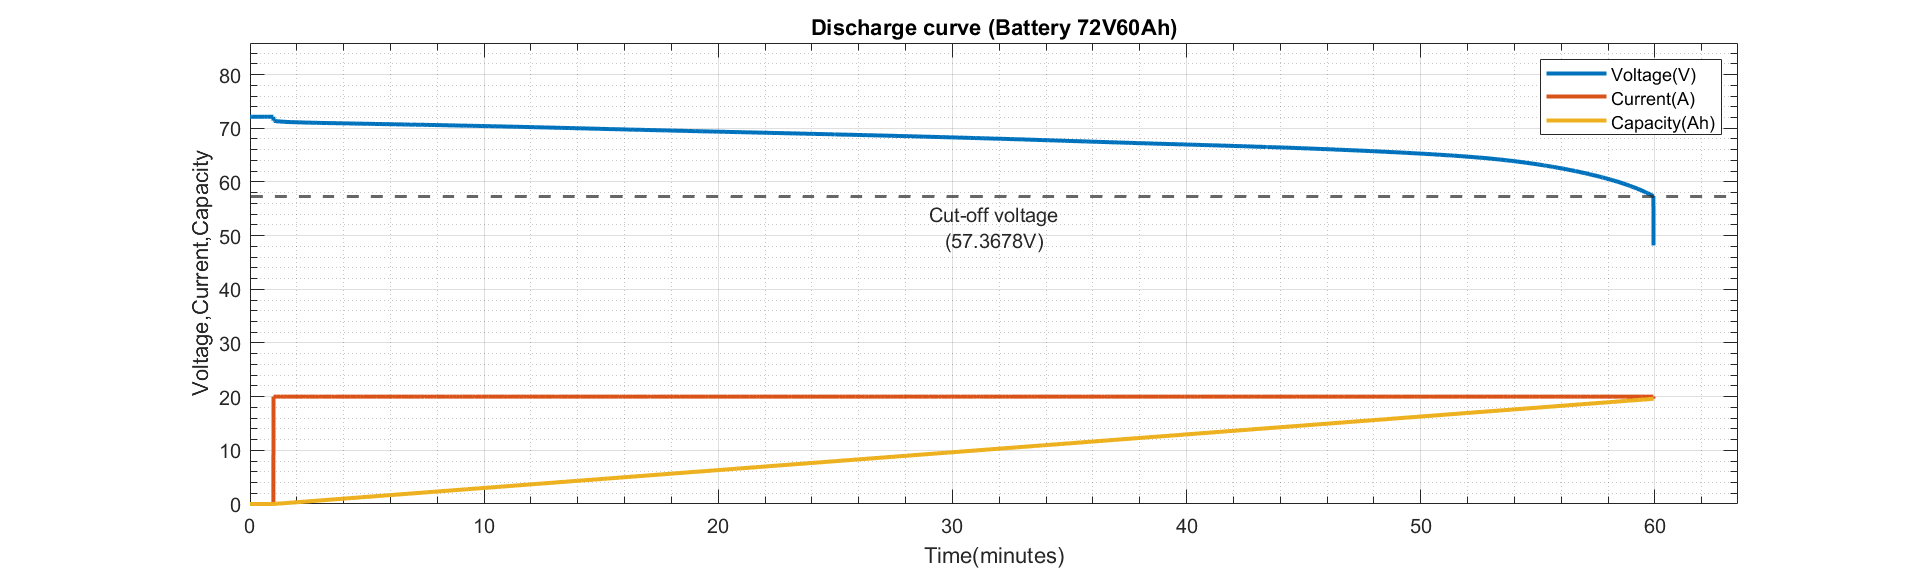
\includegraphics[width=\paperwidth]{Chapters/img/Result/Discharge curve 72V60Ah.png}}
		\centering
		\captionsetup{justification=centering,margin=2cm}
		\caption{กราฟการทดสอบการป้องกันการดิสชาร์จเกินของแบตเตอรี่ 72V60Ah}
	\end{figure}
\end{center}
จากการทดสอบพบว่าแบตเตอรี่สำหรับรถสามล้อไฟฟ้าระหว่างการทดสอบไม่มีการรั่วไหลของอิเล็ก-โทรไลต์ ไม่มีการแตกหักหรือฉีกขาด ไม่เกิดเพลิงไหม้ และไม่เกิดการระเบิด
โดยการทดสอบการดิส-ชาร์จนี้ถูกขัดจังหวะโดยระบบการจัดการแบตเตอรี่(BMS)ของโมดูลแบตเตอรี่นี้เองโดยขัดจังหวะเมื่อแรงดันของโมดูลแบตเตอรี่อยู่ที่ 57.3678V 
หลังจากที่หยุดการชาร์จจากนั้นผู้ทดสอบได้ทำการสังเกตแบตเตอรี่เป็นระยะเวลา 1 ชั่วโมงพบว่าแบตเตอรี่ยังคงสภาพปกติและยังคงสามารถใช้งานได้ซึ่งโมดูลแบตเตอรี่นี้ไม่ทราบข้อมูลคุณสมบัติอย่างชัดเจนทำให้
ไม่สามารถทราบได้ถึงความถูกต้องของแรงดันที่ระบบการจัดการแบตเตอรี่ต้องขัดจังหวะการดิสชาร์จซึ่งโดยหลังจากการทดสอบโมดูลแบตเตอรี่นี้ตามมาตรฐาน UN ECE R136 ในหัวข้อการทดสอบการป้องกันการดิสชาร์จเกิน
พบว่าโมดูลแบตเตอรี่นี้ผ่านการทดสอบโดยที่โมดูลแบตเตอรี่นี้ยังสามารถใช้งานได้อย่างปกติ
%=====================================================================================================
\newpage
ผลจากการทดสอบแบตเตอรี่ 72V 72Ah มีดังนี้
\begin{center}
	\begin{figure}[H]
	\makebox[\textwidth]{
	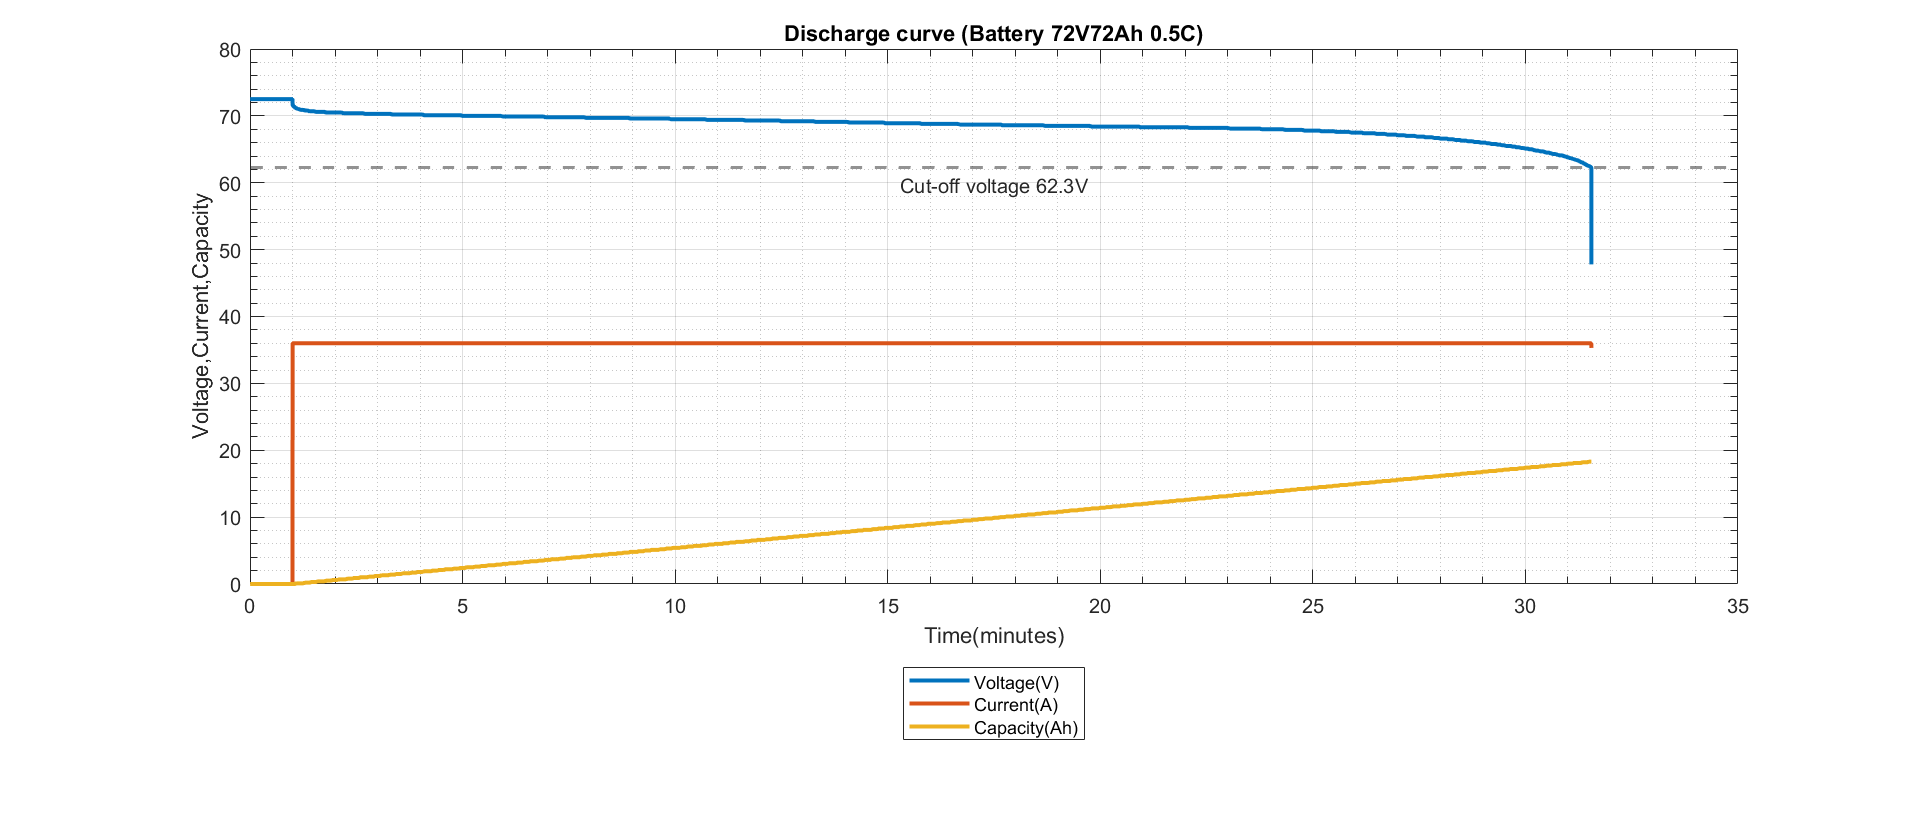
\includegraphics[width=\paperwidth]{Chapters/img/Result/Discharge curve 0.5C 72V72Ah.png}}
		\centering
		\captionsetup{justification=centering,margin=2cm}
		\caption{กราฟการทดสอบการป้องกันการดิสชาร์จเกินของแบตเตอรี่ 72V72Ah}
	\end{figure}
\end{center}
จากการทดสอบพบว่าแบตเตอรี่สำหรับรถสามล้อไฟฟ้าระหว่างการทดสอบไม่มีการรั่วไหลของอิเล็ก-โทรไลต์ ไม่มีการแตกหักหรือฉีกขาด ไม่เกิดเพลิงไหม้ และไม่เกิดการระเบิด
โดยการทดสอบการดิส-ชาร์จนี้ถูกขัดจังหวะโดยระบบการจัดการแบตเตอรี่(BMS)ของโมดูลแบตเตอรี่นี้เองโดยขัดจังหวะเมื่อแรงดันของโมดูลแบตเตอรี่อยู่ที่ 62.3V 
หลังจากที่หยุดการชาร์จจากนั้นผู้ทดสอบได้ทำการสังเกตแบตเตอรี่เป็นระยะเวลา 1 ชั่วโมงพบว่าแบตเตอรี่ยังคงสภาพปกติและยังคงสามารถใช้งานได้ซึ่งระบบการจัดการแบตเตอรี่ของโมดูลนี้จะต้องขัดจังหวะการดิสชาร์จที่
$2.3\pm 0.05V$ ต่อเซลล์(โดยแบตเตอรี่โมดูลนี้มี 22 เซลล์)หรือก็คือ $50.6\pm 1.1V$ สำหรับโมดูลแบตเตอรี่นี้ตามตารางคุณสมบัติดังรูปที่\ref{fig:BMS_Setting2}
จะเห็นได้ว่าคลาดเคลื่อนอยู่ที่ $11.7\pm 1.1V$ ซึ่งถือว่าคลาดเคลื่อนไปมากซึ่งส่งผลให้ช่วงความจุการใช้งานของโมดูลแบตเตอรี่นี้ลดลงแต่สำหรับการทดสอบตามมาตรฐาน UN ECE R136 ในหัวข้อการทดสอบการป้องกันการดิสชาร์จเกินจะสังเกตุได้ว่าโมดูลแบตเตอรี่นี้ผ่านการทดสอบโดยทีี่ยังสาามารถใช้งานได้อย่างปกติ
%=====================================================================================================
\section{ผลการทดสอบอื่นๆ}
\subsection{ผลการทดสอบการวัดความต้านทานภายในของแบตเตอรี่}
จากรูป\ref{fig:DCIR_Test}ซึ่งเป็นกราฟการทดสอบการวัดความต้านทานภายในของโมดูลแบตเตอรี่ 72V72Ah ซึ่งทดสอบขณะที่โมดูลแบตเตอรี่มีแรงดันขณะสภาวะไม่มีโหลดที่ 72V และเริ่มทดสอบด้วย
การดิสชาร์จที่อัตรากระแส 0.2C เป็นระยะเวลา 10 วินาทีและจากนั้นจึงดิสชาร์จด้วยอัตรากระแส 1C เป็นระยะเวลา 1 วินาทีโดยผลการทดสอบนี้ทำให้ได้ค่าความต้านทานภายในของแบตเตอรี่โมดูลนี้อยู่ที่
$26.8m\Omega$
\begin{center}
	\begin{figure}[H]
	\makebox[\textwidth]{
	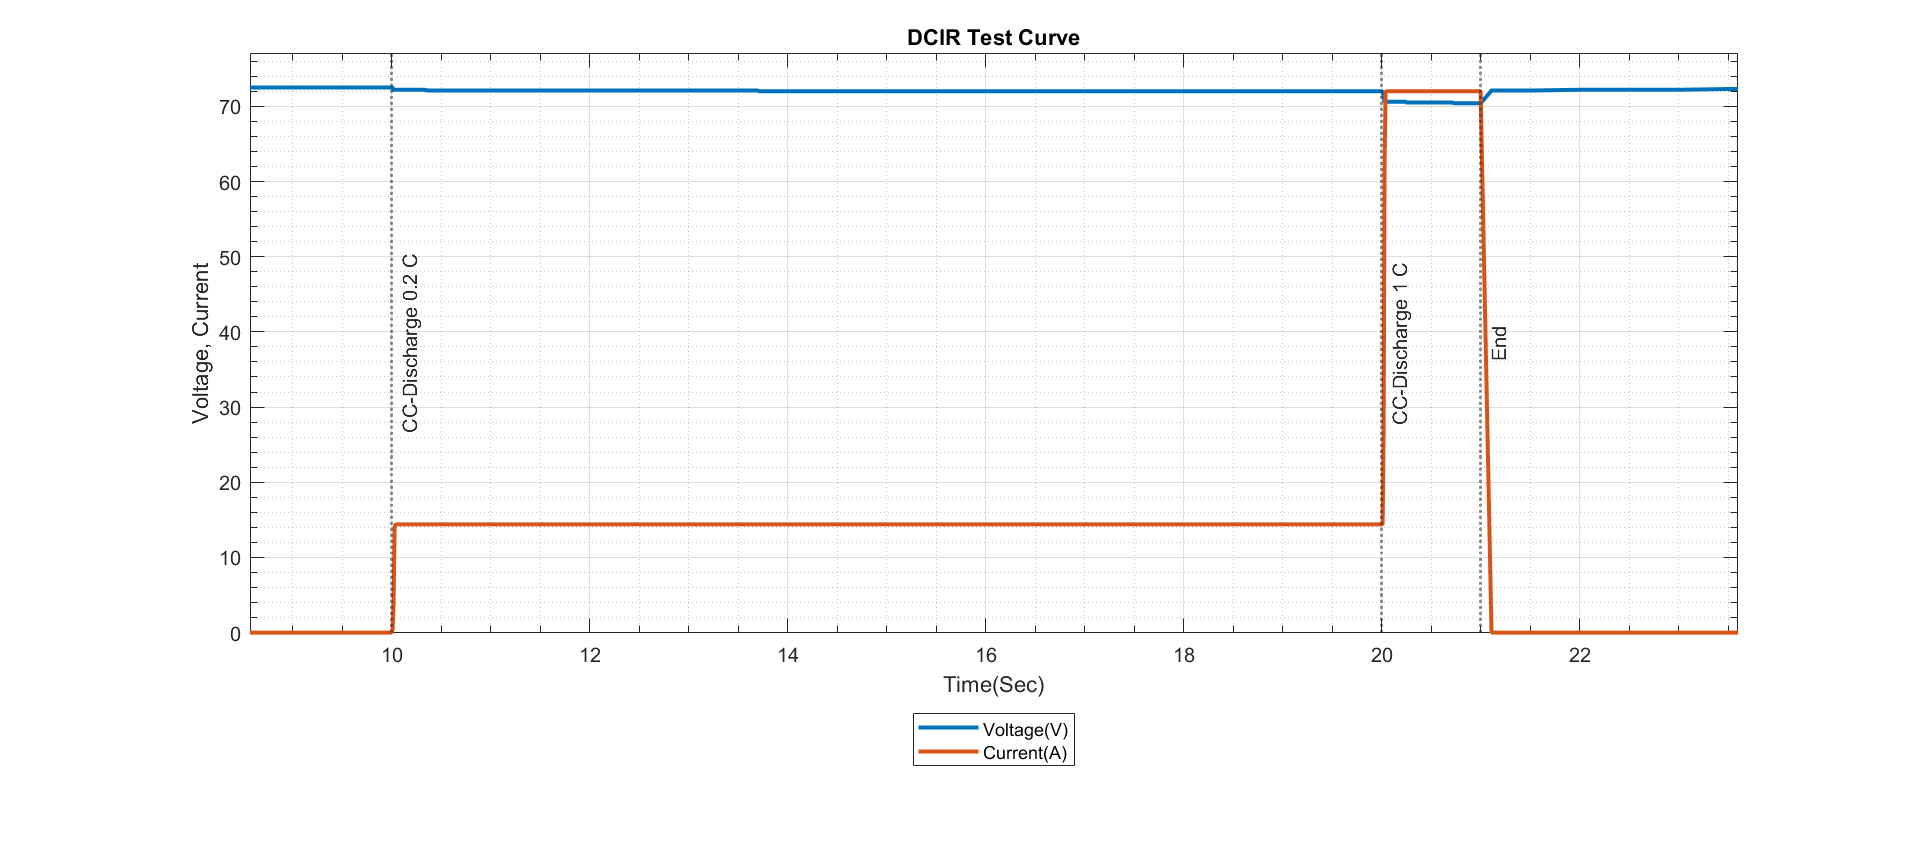
\includegraphics[width=\paperwidth]{Chapters/img/Result/DCIR_TEST.png}}
		\centering
		\captionsetup{justification=centering,margin=2cm}
		\caption{กราฟการทดสอบการวัดความต้านทานภายในของแบตเตอรี่ 72V72Ah}
		\label{fig:DCIR_Test}
	\end{figure}
\end{center}
%----------------------------------------------------------------------------------
\pagebreak
\subsection{ผลการทดสอบระยะเวลาในการพักของแบตเตอรี่}
จากรูป\ref{fig:Rest_Test} การทดสอบนี้หลังจากการดิสชาร์จที่กระแส 0.5C โดยหลังจากการดิสชาร์จแรงดันของโมดูลแบตเตอรี่นี้อยู่ที่ 66.5V 
และเมื่อทำการวัดแรงดันของโมดูลแบตเตอรี่นี้พบว่าแรงดันจะเพิ่มขึ้นทีละน้อยเมื่อระยะเวลาผ่านไปโดยประมาณ 30 นาทีแรงดันจึงไม่เกิดการเปลี่ยนแปลงซึ่งแนวโน้มผลการทดสอบนี้มีแนวโน้มใกล้เคียงกับงานวิจัย\cite{9209879}
\begin{center}
	\begin{figure}[H]
	\makebox[\textwidth]{
	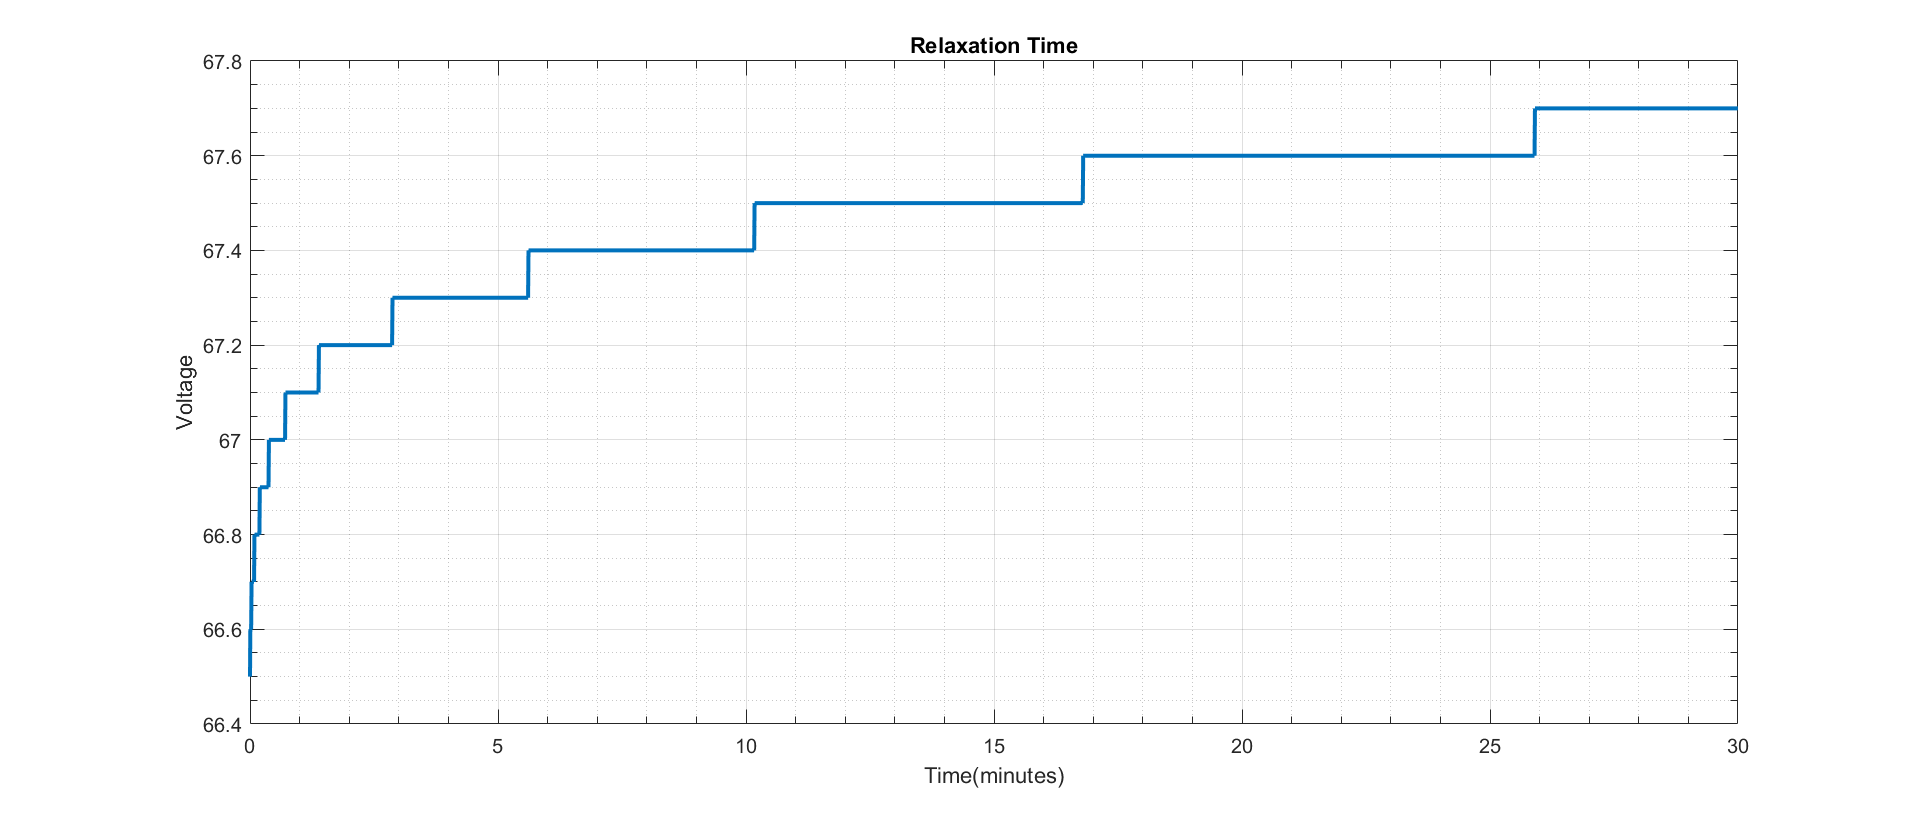
\includegraphics[width=\paperwidth]{Chapters/img/Result/Relaxation Time.png}}
		\centering
		\captionsetup{justification=centering,margin=2cm}
		\caption{กราฟการทดสอบระยะเวลาพักแบตเตอรี่ 72V72Ah}
		\label{fig:Rest_Test}
	\end{figure}
\end{center}
%----------------------------------------------------------------------------------
\pagebreak
\subsection{ผลการทดสอบอัตรากระแส}
จากรูป\ref{fig:C_rate_Test} การทดสอบอัตรากระแสนี้ได้จากการทดสอบดิสชาร์จแบตเตอรี่ 72V72Ah ด้วยอัตรากระแส 0.3C เทียบกับอัตรากระแส 0.5C ซึ่งจะเห็นได้ว่าและความจุจากการที่ดิสชาร์จ
ด้วยอัตรากระแสที่มากกว่าทำให้แรงดันนั้นลดลงรวดเร็วมากกว่าการดิสชาร์จด้วยอัตรากระแสที่น้อยกว่าเช่นเดียวกับความจุที่ลดลงอย่างรวดเร็วเช่นเดียวกันซึ่งขณะที่ทดสอบแบตเตอรี่มีแรงดันอยู่ที่ 72V
\begin{center}
	\begin{figure}[H]
	\makebox[\textwidth]{
	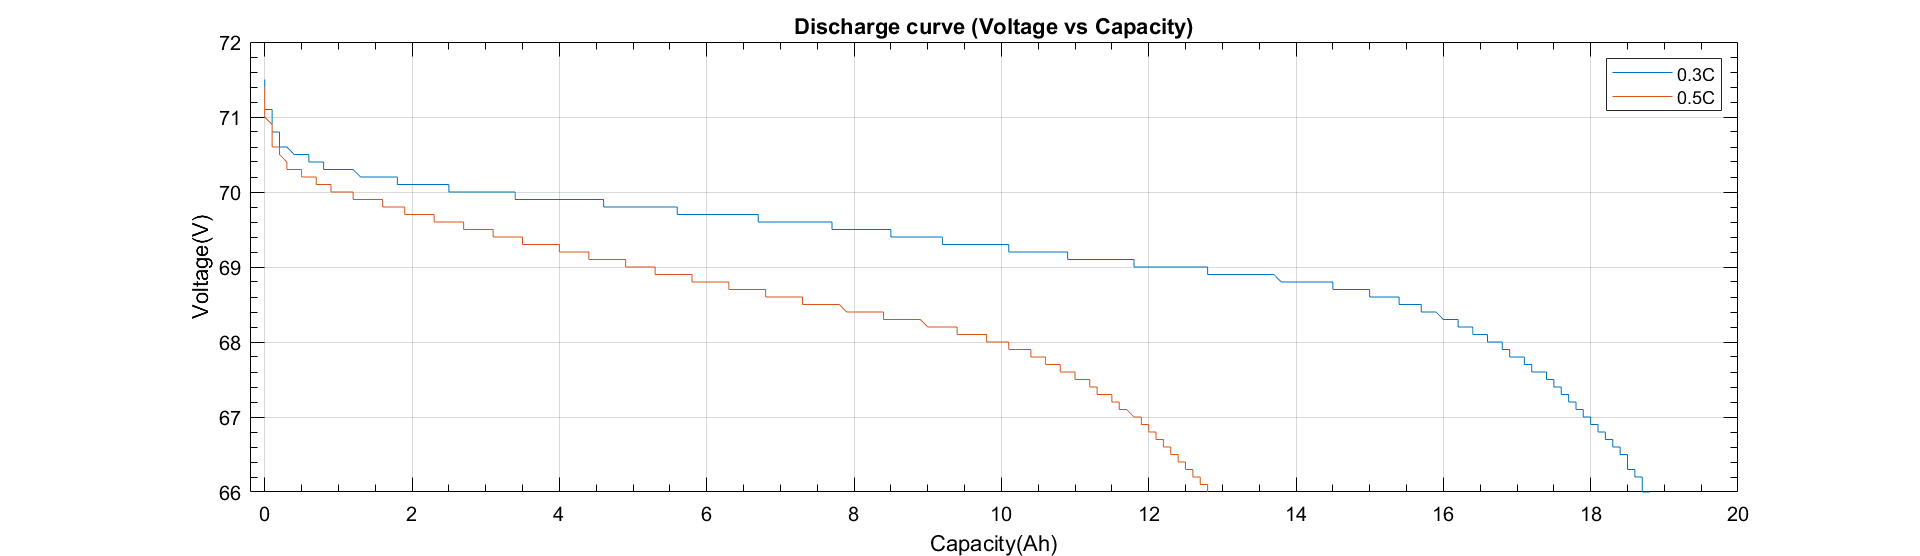
\includegraphics[width=\paperwidth]{Chapters/img/Result/Discharge curve V vs Ah.png}}
		\centering
		\captionsetup{justification=centering,margin=2cm}
		\caption{กราฟการทดสอบอัตรากระแสดิสชาร์จ 72V72Ah}
		\label{fig:C_rate_Test}
	\end{figure}
\end{center}